\section{Mathematical Notation, Set Theory, and Functions}

We begin by reviewing standard mathematical notation,
the basics of set theory, and \glspl{function}.

\subsection{Introduction to Set Theory}

We use ``$\mathDef{}$'' when making definitions.
Thus,

\begin{equation}
    a \mathDef{} b
\end{equation}

\noindent
means that we \emph{define} $a$ as $b$ and may be read as
``$a$ is (defined to be) $b$''.

For our purposes, a \emph{\gls{set}} is a collection of elements or objects.
We suppose that $A$ is a \gls{set}.
If $a$ is an element of $A$, we write $a\in A$;
this may be read as ``$a$ is an element of $A$'' or ``$a$ is in $A$''.
If $a$ is not an element of $A$, we write $a\notin A$;
this may be read as ``$a$ is not an element of $A$'' or ``$a$ is not in $A$''.
We will always have that $a\in A$ or $a\notin A$
for all sets $A$ and elements $a$.
The \gls{set} which contains no elements $\braces{}$
is called the \emph{empty set}
and is denoted by $\emptyset$.

If the sets $A$ and $B$ contain the same elements,
then they denote the same set and we write $A = B$;
this may be read as ``$A$ equals $B$''.
Otherwise, $A$ and $B$ do not contain the same elements,
and we write $A\ne B$;
this may be read as ``$A$ does not equal $B$''.

If $B$ is a set and for every $b\in B$ we have $b\in A$, then $B$ is a subset
of $A$ and we write $B\subseteq A$.
We may read $B\subseteq A$ as ``$B$ is a subset of $A$''.
If $B$ is a subset of $A$ and $B$ is not equal to $A$,
then $B$ is a proper subset of $A$;
in this case, $B\subseteq A$ and there is some $a\in A$ such that $a\notin B$.
We may write this as $B\subset A$;
this may be read as ``$B$ is a proper subset of $A$''.
Given any set $A$, we always have that the empty set is a subset of $A$:
$\emptyset\subseteq A$.

Starting with one \gls{set}, we would like to make other \glspl{set}.
Let $X$ be a set and $P$ is some property that
elements of $X$ may or may not have.
If we want to define a new set $A$ as the set of all elements
in $X$ which have property $P$, we would write

\begin{equation}
    A \mathDef{} \braces{x\in X\mid P}.
\end{equation}

\noindent
This is ``set builder'' notation.
We should read $A \mathDef{} \braces{x\in X\mid P}$ as
``$A$ is (defined to be) the set of all $x$ in $X$ such that
(property) $P$ is true''.
Here, we use ``$\mid$'' as a separator that should be read as ``such that.''
When using set builder notation, the overall set $X$ may not always
be explicitly stated.

Within set builder notation, we may use ``$\exists$'' as shorthand
for ``there exists'' or ``there is'';
we may also use ``$\forall$'' as shorthand for ``for all''.
Outside of set builder notation, we will try to not use this shorthand.

We will be interested in operations between sets,
and we will want to combine them in various ways.
Let $A$ and $B$ be sets.
We have the following definitions:

\begin{align}
    A \cup B &\mathDef{} \braces{x \mid x\in A \text{ or } x\in B}
        \nonumber\\
    A \cap B &\mathDef{} \braces{x \mid x\in A \text{ and } x\in B}
        \nonumber\\
    A \setminus B &\mathDef{} \braces{a\in A \mid a\notin B}.
    \label{eq:math_set_theory_basic_set_ops}
\end{align}

\noindent
Thus, $A\cup B$ contains elements that are in $A$ or $B$;
this should be read ``$A$ union $B$''.
$A\cap B$ is the set containing elements that are in both $A$ and $B$;
this should be read ``$A$ intersect $B$''.
$A\setminus B$ is the set containing elements in $A$ that are not in $B$;
this could be read ``$A$ set minus $B$'' or ``$A$ minus $B$''.
See Figure~\ref{fig:math_set_venn} for a graphical representation
of these set operations.

\begin{figure}[t]
\centering
    \begin{subfigure}[t]{0.45\textwidth}
    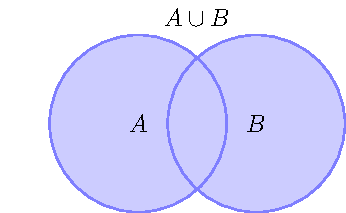
\includegraphics[width=\textwidth]{figures/math/set_theory/set_venn_or.pdf}
    \end{subfigure}
    \begin{subfigure}[t]{0.45\textwidth}
    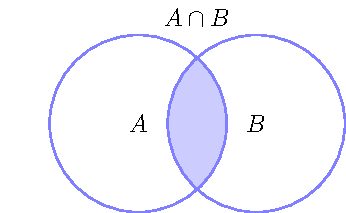
\includegraphics[width=\textwidth]{figures/math/set_theory/set_venn_and.pdf}
    \end{subfigure}

    \begin{subfigure}[t]{0.45\textwidth}
    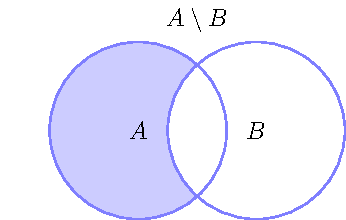
\includegraphics[width=\textwidth]{figures/math/set_theory/set_venn_minus.pdf}
    \end{subfigure}

    \caption[Set operations]{Here is a figure of various set operations:
        set union, set intersection, and set minus.
        Modified from the example
        \href{https://texample.net/tikz/examples/set-operations-illustrated-with-venn-diagrams/}{here}.}
    \label{fig:math_set_venn}
\end{figure}


\begin{example}[Examples of Sets and Set Operations]
We have the following definitions:

\begin{align}
    A &\mathDef{} \braces{0, 1, 2, 3}
        \nonumber\\
    B &\mathDef{} \braces{1, 2, 3, 4}
        \nonumber\\
    C &\mathDef{} \braces{1, 2, 3}
        \nonumber\\
    D &\mathDef{} \braces{1, 3, 5, 7}.
\end{align}

\noindent
Then we see

\begin{align}
    A \cup B &= \braces{0, 1, 2, 3, 4} \nonumber\\
    A \cap B &= \braces{1, 2, 3} \nonumber\\
        &= C \nonumber\\
    A \setminus B &= \braces{0}.
\end{align}

\noindent
We also note that all of the elements in $C$ are also in $A$ and $B$;
this implies that

\begin{align}
    C &\subseteq A
        \nonumber\\
    C &\subseteq B.
\end{align}

\noindent
Because $C\ne A$ and $C\ne B$, we have

\begin{align}
    C &\subset A
        \nonumber\\
    C &\subset B.
\end{align}

\noindent
Finally, we have

\begin{align}
    (A \cup C) \cup D &= \braces{0, 1, 2, 3, 5, 7} \nonumber\\
    (A \cap C) \cap D &= \braces{1, 3} \nonumber\\
    C \setminus D &= \braces{2} \nonumber\\
    C \setminus B &= \emptyset.
\end{align}
\end{example}

A further discussion of set theory may be found in
Appendix~\ref{app:math_set_theory}.

\subsection{Standard Mathematical Sets}
\label{ssec:standard_math_sets}

We have the following standard definitions for common collections
of numbers:

\begin{align}
    \N &\mathDef{} \braces{0, 1, 2, \ldots} \nonumber\\
    \Z &\mathDef{} \braces{\ldots, -2, -1, 0, 1, 2, \ldots} \nonumber\\
    \Q &\mathDef{} \braces{a/b \mid a,b\in\Z, b\ne0} \nonumber\\
    \R &\mathDef{} \braces{\text{the set of all real numbers}} \nonumber\\
    \C &\mathDef{} \braces{a + bi \mid a,b\in\R}.
\end{align}

\noindent
Naturally, we have the naturals $\N$, the integers $\Z$,
the rational numbers $\Q$, the real numbers $\R$,
and the complex numbers $\C$.

We also have the following standard definitions.
Not all of these will make sense at this time because
not everything has been defined.
We will discuss them in more detail in later chapters.

\begin{align}
    n\Z &\mathDef{} \braces{\ldots, -2n, -n, 0, n, 2n, \ldots}, \quad n\ge1
        \nonumber\\
    \Z_{n} &\mathDef{} \braces{0, 1, 2, \ldots, n-1}, \quad n>1\nonumber\\
    \Z_{n}^{*} &\mathDef{} \braces{a\in\Z_{n}\mid \gcd(a,n)=1}
        \nonumber\\
    \F_{p} &\mathDef{} \braces{0, 1, 2, \cdots, p-1}, \quad \text{$p$ prime}
        \nonumber\\
    \F_{p}^{*} &\mathDef{} \F_{p}\setminus\braces{0} \nonumber\\
    \braces{0,1}^{n} &\mathDef{} \braces{\text{The set of all $n$-bit strings}}
        \nonumber\\
    \braces{0,1}^{*} &\mathDef{}
        \braces{\text{The set of all finite bit strings}}.
\end{align}

\begin{example}[More Examples of Sets and Set Operations]
From the definitions, we see

\begin{align}
    \Z \cup \N &= \Z \nonumber\\
    \Z \cap \N &= \N \nonumber\\
    \Z \setminus \N &= \braces{\ldots, -3, -2, -1} \nonumber\\
    \Z \setminus \Q &= \emptyset.
\end{align}

\noindent
Additionally, for all sets $A$, we always have

\begin{align}
    A \cup \emptyset &= A \nonumber\\
    A \cap \emptyset &= \emptyset.
\end{align}
\end{example}

We write $a\chooseRandom{}A$ to denote that $a$ is chosen uniformly
at random from the \gls{set} $A$;
in this case, we assume that $A$ has a finite number of elements.

\subsection{Functions}

We will look at \glspl{function} between \glspl{set}.
Let $A$ and $B$ be \glspl{set}.
A \emph{\gls{function}} $f:A\to B$ uniquely assigns every element in
$a\in A$ to some element in $B$.
More specifically, for all $a\in A$ we have $f(a)\in B$.
We should read $f:A\to B$ as ``(a function) $f$ from $A$ to $B$''.
We say that $A$ is the \emph{domain} of $f$
and $B$ is the \emph{codomain} of $f$.
The \emph{range} of $f$ is defined to be $f(A)$:

\begin{equation}
    f(A) \mathDef{} \braces{b\in B \mid \exists a\in A, f(a) = b}.
    % TODO: possibly change to
    %       \braces{f(a)\in B \mid a\in A}.
\end{equation}

\noindent
This definition can be read as ``$f(A)$ is the set of all $b\in B$
such that there is an $a\in A$ so that $f(a) = b$''.
In this way, the range is everything that $f$ ``hits'':
if $\bar{b}\in f(A)$, then there is some $\bar{a}\in A$ with
$f(\bar{a}) = \bar{b}$.

\begin{example}[Example of a Function]
\label{example:function}
We let $A = \braces{0, 1, 2, 3}$ and $B = \braces{1, 2, 3, 4}$.
We define a \gls{function} $f:A\to B$ as follows:

\begin{align}
    f(0) &\mathDef{} 1 \nonumber\\
    f(1) &\mathDef{} 2 \nonumber\\
    f(2) &\mathDef{} 3 \nonumber\\
    f(3) &\mathDef{} 2.
\end{align}

\noindent
While we may sometimes think of \glspl{function} in terms of their graphs
like in Figure~\ref{fig:parabola_plot},
in this case we have fully specified $f$ by assigning every element in $A$
to some element in $B$;
thus, $f$ is a \gls{function}.

We see that

\begin{equation}
    f(A) = \braces{1,2,3} \subset B.
\end{equation}

\noindent
We have $1\in f(A)$ because $f(0) = 1$;
$2\in f(A)$ because $f(3) = 2$; and
$3\in f(A)$ because $f(2) = 3$.
Thus, the range $f(A)$ is a proper subset of the codomain $B$.
\end{example}

\begin{example}[Another Example of a Function]
We now have a more standard example of a \gls{function}.
We recall that $\R$ denotes the set of real numbers.

\begin{figure}[t]
\centering
    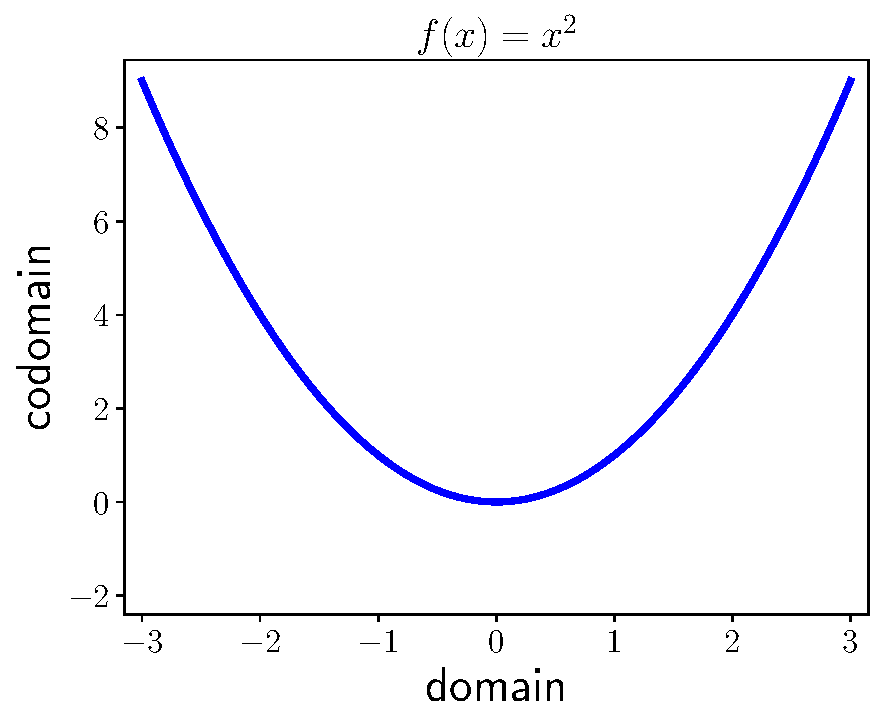
\includegraphics[width=10cm]{plots/parabola/function_parabola.pdf}
    \caption[Plot of a parabola]{Here
        we have a plot of the \gls{function} $f:\R\to\R$ with $f(x) = x^{2}$:
        the standard parabola.
        The domain of $f$ is the real numbers $\R$;
        the codomain of $f$ is also $\R$.
        We have that the range of $f$ is the \gls{set} of nonnegative
        real numbers: $f(\R) = [0,\infty)$.
        }
    \label{fig:parabola_plot}
\end{figure}


Let $f:\R\to\R$ and set $f(x) = x^{2}$.
In this case, the domain of the \gls{function} is $\R$
and the codomain of the \gls{function} is $\R$.
In this case, the range $f(\R) = [0,\infty)$.
We know the graph of $f$ is the standard parabola;
see Figure~\ref{fig:parabola_plot}.
\end{example}

\subsection{Function Properties}

We now list some standard properties that \glspl{function} may have:

\begin{itemize}
\item A \gls{function} $f:A\to B$ is \emph{\gls{injective}}
    or \emph{one-to-one} if $f(x) = f(y)$ implies that $x = y$.
    Equivalently, $f$ is injective if $x\ne y$ implies that $f(x) \ne f(y)$.
\item A \gls{function} $f:A\to B$ is \emph{\gls{surjective}} or \emph{onto}
    if for every $b\in B$ there is an $a\in A$ such that $f(a) = b$.
    This means that the range is equal to the codomain: $f(A) = B$.
\item A \gls{function} $f:A\to B$ is \emph{\gls{bijective}}
    (or $f$ is a \emph{bijection})
    if $f$ is both \gls{injective} and \gls{surjective}.
    In this case, $f$ has an \emph{inverse function} $g:B\to A$
    which satisfies

\begin{equation}
    g(f(a)) = a
\end{equation}

\noindent
and

\begin{equation}
    f(g(b)) = b
\end{equation}

\noindent
for all $a\in A$ and $b\in B$.
\end{itemize}

\begin{example}
The \gls{function} $f$ in Example~\ref{example:function}
is not \gls{injective}, \gls{surjective}, or \gls{bijective}.

\begin{itemize}
\item $f$ is not \gls{injective} because $f(1) = f(3) = 2$ but $1\ne3$.
\item $f$ is not \gls{surjective} because no element is mapped to $4\in B$.
\item $f$ is not \gls{bijective} because it is not
    \gls{injective} and \gls{surjective}.
\end{itemize}
\end{example}

\noindent
In preparation for more examples, we define the following functions:

\begin{align}
    f:\N\to\N,\quad &f(n) \mathDef{} n+1 \nonumber\\
    g:\Z\to\Z,\quad &g(n) \mathDef{} n+1 \nonumber\\
    h:\R\to\R,\quad &h(x) \mathDef{} x^{2}.
    \label{eq:math_set_theory_function_property_example_funcs}
\end{align}



\begin{example}[Injective Functions 1: Example]
\label{example:injective_functions_1}
We use the \gls{function} $f$ as defined in
Eq.~\eqref{eq:math_set_theory_function_property_example_funcs}.

If we have $n,m\in\N$ with

\begin{equation}
    f(n) = f(m),
\end{equation}

\noindent
this implies that

\begin{equation}
    n+1 = m+1,
\end{equation}

\noindent
so $n = m$.
Thus, $f$ is \gls{injective}.
\end{example}

\begin{example}[Injective Functions 2: Example]
\label{example:injective_functions_2}
We use the \gls{function} $g$ as defined in
Eq.~\eqref{eq:math_set_theory_function_property_example_funcs}.

Using the same argument from Example~\ref{example:injective_functions_1},
we see that $g$ is \gls{injective}.
\end{example}

\begin{example}[Injective Functions 3: Non-example]
\label{example:injective_functions_3}
We use the \gls{function} $h$ as defined in
Eq.~\eqref{eq:math_set_theory_function_property_example_funcs}.

For $x>0$, we see that $f(x) = f(-x)$ with $x\ne -x$.
In particular, we have $f(1) = f(-1) = 1$ but $1\ne-1$.
Thus, $h$ is not \gls{injective}.
\end{example}



\begin{example}[Surjective Functions 1: Non-example]
\label{example:surjective_functions_1}
We see that $f$ is not \gls{surjective},
because $0\in\N$ and there is no $n\in\N$ such that $f(n) = 0$.
\end{example}

\begin{example}[Surjective Functions 2: Example]
\label{example:surjective_functions_2}
Given $n\in\Z$, we see that $n-1\in\Z$ and

\begin{equation}
    g(n-1) = n.
\end{equation}

\noindent
Thus, $g$ is \gls{surjective}.
\end{example}

\begin{example}[Surjective Functions 3: Non-example]
\label{example:surjective_functions_3}
We see that $h$ is not \gls{surjective}.
This is because we know that for $x\in\R$, we have

\begin{equation}
    h(x) = x^{2}\ge0.
\end{equation}

\noindent
In particular, $-1\in\R$ yet there is no $x\in\R$ such that $h(x) = -1$.
\end{example}



\begin{example}[Bijective Functions 1: Non-example]
\label{example:bijective_functions_1}
In Example~\ref{example:injective_functions_1}
we showed that $f$ is \gls{injective}
while Example~\ref{example:surjective_functions_1}
showed that $f$ is not \gls{surjective};
thus, $f$ is not \gls{bijective}.
\end{example}

\begin{example}[Bijective Functions 2: Example]
\label{example:bijective_functions_2}
In Example~\ref{example:injective_functions_2}
we showed that $g$ is \gls{injective}
while Example~\ref{example:surjective_functions_2}
showed that $g$ is \gls{surjective};
thus, $g$ is \gls{bijective}.
\end{example}

\begin{example}[Bijective Functions 3: Non-example]
\label{example:bijective_functions_3}
In Example~\ref{example:injective_functions_3}
we showed that $h$ is not \gls{injective}
while Example~\ref{example:surjective_functions_3}
showed that $h$ is not \gls{surjective};
thus, $h$ is not \gls{bijective}.
\end{example}



\subsection{Permutations}

\Glspl{permutation} are a specific type of \gls{function};
in particular, \glspl{permutation} are bijections from a \gls{set} to itself.
More formally, if $A$ is a \gls{set},
the \gls{function} $f:A\to A$ is a \emph{\gls{permutation}}
if $f$ is \gls{bijective}.

\begin{example}[Permutations: Examples]
We let $A = \braces{1,2,3,4}$.

We define $f:A\to A$ by

\begin{align}
    f(1) &\mathDef{} 2
        \nonumber\\
    f(2) &\mathDef{} 3
        \nonumber\\
    f(3) &\mathDef{} 4
        \nonumber\\
    f(4) &\mathDef{} 1.
\end{align}

\noindent
Here, we see that $f$ is a \gls{permutation}.

Similarly, we can define $g:A\to A$ by

\begin{align}
    g(1) &\mathDef{} 4
        \nonumber\\
    g(2) &\mathDef{} 1
        \nonumber\\
    g(3) &\mathDef{} 2
        \nonumber\\
    g(4) &\mathDef{} 3.
\end{align}

\noindent
Here, $g$ is also a \gls{permutation}.
We can see that

\begin{align}
    f(g(1)) &= 1
        \nonumber\\
    f(g(2)) &= 2
        \nonumber\\
    f(g(3)) &= 3
        \nonumber\\
    f(g(4)) &= 4.
\end{align}

\noindent
Naturally, this formally shows that $f$ and $g$ are inverses.
\end{example}

\begin{example}[Permutations: Non-example]
As before, we let $A = \braces{1,2,3,4}$.

We define $h:A\to A$ by

\begin{align}
    h(1) &\mathDef{} 2
        \nonumber\\
    h(2) &\mathDef{} 3
        \nonumber\\
    h(3) &\mathDef{} 4
        \nonumber\\
    h(4) &\mathDef{} 4.
\end{align}

\noindent
We see that $h$ is not a \gls{permutation} because it is not a bijection.
In particular, $h$ is not \gls{injective} because $3,4\in A$
with $h(3) = h(4)$ yet $3\ne4$.
\end{example}
